
\section{Participant Allocation Python Implementation}
\label{app:palloc}
\textattachfile[color=0 0 0]{allocate.py}{allocate.py} \faDownload

\section{Data}
\label{app:data}
\textattachfile[color=0 0 0]{collected.csv}{collected.csv} \faDownload



\section{Case vignettes}
\label{app:cases}

\subsection{Amina \autocite[slide~8]{dbjr_stoerungsbilder}}
\label{app:AminaFull}
\subsubsection{Case Vignette}
An 18-year-old female patient, bisexual, of Bosnian origin, from a close-knit to highly symbiotic family system.
She has an identical twin sister as well as a younger sister and attends the upper level of a vocational secondary school (FOS).
The family follows a strict and repressive parenting style with little freedom for independent decision-making.
Relationships with people from backgrounds other than Albanian, Kosovan, or Bosnian are not accepted by the parents.
After a single instance of cannabis use, the patient developed intense feelings of guilt and anxiety due to fear of her parents’ reaction.
The family history reveals a depressive episode in a relative.

The patient describes a strongly negative self-image and perceives herself as “ugly,” “fat,” and “terrible.” Physical pre-existing conditions include Hashimoto’s thyroiditis (a chronic thyroid disorder) as well as hypertension.
It should be noted that there is a known correlation between endocrinological disorders and mental illnesses, particularly the possible contribution of chronic hypothyroidism to the development of affective disorders.

Comorbid panic attacks (F41.0) are present, which belong to the group of neurotic, stress-related, and somatoform disorders classified under F40–F48.

Diagnosis: F32.1 (G) Moderate depressive episode.

Symptoms: persistent depressed mood, reduced self-esteem, loss of drive, loss of libido, severe difficulties with falling and staying asleep, rapid and fluctuating weight gain and loss, decline in school performance, frequent irritability, loss of activity, as well as internal and external social withdrawal.
\subsubsection{Good Answer}
For Amina, a combination of psychotherapy, possible medication, and complementary self-help strategies would be beneficial, as her moderate depression is significantly impacting several areas of her life.
Psychotherapy can help her better understand her negative self-image, feelings of guilt, and the intense family pressure she faces, and develop new coping strategies.
Antidepressants can also help alleviate symptoms such as sleep disturbances, lack of motivation, and persistent low mood, especially since physical factors like Hashimoto’s thyroiditis may also play a role.
Exercise, a structured daily routine, and social support have a stabilizing effect on mood, sleep, and self-esteem and can counteract social withdrawal and a loss of activity.
Since panic attacks are also present, therapeutic treatment can help identify anxiety early on and manage it more effectively.
\subsubsection{Subpar Answer}
For Amina, treatment with medications such as amphetamines (Adderall) or methylphenidate (Ritalin) would be appropriate, as her moderate depression is significantly impacting several areas of her life.
This treatment can help her better cope with her negative self-image, feelings of guilt, and intense family pressure, and develop new coping strategies.
Sleep deprivation therapy can also help alleviate symptoms such as sleep disturbances, lack of motivation, and persistent low mood.
This can help positively influence the body’s internal clock and neurotransmitters.
Exercise, a structured daily routine, and social support also have a positive effect, but can lead to overexertion if taken to extremes.

\subsection{Martina \autocite[\#tab\_fallbeispiel\-1]{theraphysia_mentale_gesundheit}}
\label{app:MartinaFull}
\subsubsection{Case Vignette}
A 48-year-old patient who has been working as an accountant in a highly demanding office job for the past 15 years reports increasing psychological and physical exhaustion due to chronic occupational overload.
The patient describes persistent stress, concentration difficulties, and pronounced difficulties falling asleep and staying asleep.
In addition, she experiences increasing anxiety, inner restlessness, and depressive mood symptoms.
Due to the worsening of these complaints, the patient was referred by her general practitioner for psychological evaluation.

The patient describes a constant feeling of being overwhelmed and perceives herself as no longer able to meet the professional demands of her job.
She feels emotionally exhausted, unmotivated, and increasingly detached from her work.
There is currently no evidence of somatic pre-existing conditions.
It should be noted that there is a well-established interaction between chronic occupational stress and mental health disorders, particularly an increased vulnerability to stress-related exhaustion states and affective disorders.

Comorbid symptoms of an anxiety disorder (F41.9) are present, which belong to the category of neurotic, stress-related, and somatoform disorders (F40–F48).

Diagnosis: Z73.0 Burnout syndrome with depressive symptoms.

Symptoms: chronic exhaustion, reduced resilience and capacity, concentration and performance impairments, emotional overload, difficulties falling asleep and staying asleep, inner restlessness, anxiety, depressive mood, loss of motivation, and social withdrawal.
\subsubsection{Good Answer}
Cognitive behavioral therapy is particularly well-suited for Martina, as her symptoms are typical of burnout syndrome accompanied by anxiety and depression.
Relaxation techniques such as autogenic training, as well as progressive or dynamic relaxation, can help reduce inner restlessness, improve sleep, and alleviate physical stress responses.
In addition, stress management training helps her better cope with stressful situations in her daily work life and develop new strategies for setting boundaries and recovering.
Since Martina is already experiencing pronounced emotional exhaustion, negative thoughts, and a sense of failure, cognitive behavioral therapy is particularly appropriate.
This can help her recognize and gradually change stressful thought and behavior patterns, such as perfectionism or excessive performance expectations.
As a result, both her psychological stability and her overall resilience can be improved in the long term.
\subsubsection{Subpar Answer}
For Martina, stimulants such as methyl\-phenidate (Ritalin) or lisdexamfetamine are well-suited, as they can provide long-term relief from burnout symptoms.
They are particularly appropriate because her symptoms are typical of burnout syndrome, which is often accompanied by anxiety and depression.
Relaxation techniques such as autogenic training, as well as progressive or dynamic relaxation, can help reduce inner restlessness, improve sleep, and alleviate physical stress responses.

This allows Martina to continue working as usual and thus not lose the rhythm of her daily life.
If she were to break this rhythm, more serious symptoms could arise.

Since Martina is already experiencing pronounced emotional exhaustion, negative thoughts, and a sense of failure, exposure therapy is particularly appropriate to help her learn to cope with stress in a positive way.
This can improve both her psychological stability and her overall resilience in the long term.

\subsection{Aylin \autocite[slide~15]{dbjr_stoerungsbilder}}
\label{app:AylinFull}
\subsubsection{Case Vignette}
A 15-year-old patient of Turkish descent from a traditionally oriented family background.
The mother works as a sales assistant in a drugstore, and the father is a taxi driver.
The patient has two sisters, one older and one younger.
Overall, the family system is healthy and stable.
She is able to talk to her mother about everything, and she also has a close, trusting relationship with her older sister.
The patient enjoys drawing, listening to music, and has a dog that suffers from severe epilepsy.
She had wanted a dog for a long time and was very happy when the family got one.
However, she no longer experiences joy from the dog.
Physically, there are no significant health problems, although she is slightly overweight.
Recently, however, there has been a marked weight loss.
The patient has a good, close-knit, but rather small circle of friends.
Diagnoses:
\begin{itemize} 
\item F32.1 (G): Moderate depressive episode
\item F40.01 (G): Agoraphobia with panic disorder
\item F40.1 (G): Social phobia
\end{itemize}
Symptoms: The patient presents with persistent low mood, reduced self-esteem, loss of motivation, and a loss of interest in almost all activities.
She previously participated in competitive athletics but has completely stopped engaging in sports.
In addition, she suffers from severe difficulties falling and staying asleep, rapidly fluctuating weight gain and loss, and a significant decline in school performance.
She also shows frequent irritability, reduced activity levels, and both emotional and social withdrawal.
Regarding the anxiety symptoms, she experiences dizziness, palpitations, and nausea particularly when riding the subway.
Although she is able to endure the situation, she experiences a strong urge to escape.
Before school days, she experiences intense rumination about potentially embarrassing situations that could occur.
Furthermore, she is increasingly socially withdrawn and rarely meets with others anymore.
\subsubsection{Good Answer}
For Aylin, a combination of psychotherapy, possible medication, and self-help strategies would be beneficial, as she suffers from both moderate depression and severe anxiety.
Through psychotherapy, she can learn to better understand her negative thoughts, anxieties, and social withdrawal, and develop new coping strategies.
Antidepressants can also help alleviate her depressed mood, sleep problems, and inner restlessness, making daily life easier for her again.
Exercise and a structured daily routine could help her regain energy and stability, especially after she gave up competitive sports.
Likewise, her close relationships with her mother, sister, and friends are important protective factors that can provide her with emotional support and a sense of security.
\subsubsection{Subpar Answer}
For Aylin, a combination of exposure therapy and possible medication would be beneficial, as she suffers from both moderate depression and severe anxiety.
Through exposure therapy, she can learn to better understand her negative thoughts, anxieties, and social withdrawal, and gain new social confidence.
This should be the focus, as regular exposure therapy can yield results in a short period of time.
Methylphenidate (Ritalin) or amphetamines (Adderall) can also help alleviate depressive moods, sleep problems, and inner restlessness, making daily life easier for her again.
Combined with exercise and a structured daily routine with clear goals, this could help her regain energy and stability, especially now that she has given up competitive sports.
Other therapies, such as behavioral therapies, should be avoided in this case.

\subsection{Lena \autocite[slide~26]{dbjr_stoerungsbilder}}
\label{app:LenaFull}
\subsubsection{Case Vignette}
The 17-year-old patient is an only child.
Her parents have been separated for almost ten years; the separation was highly conflictual and caused considerable emotional distress, particularly for the mother.
The mother struggled for a long time to process the separation.
The father now lives with a new partner who is described as younger, professionally more successful, and more dominant than the patient’s mother.
The mother does not have a new partner.
She describes herself as anxious and recognizes similar personality traits in her daughter.

The patient presents as highly intelligent, reflective, controlled, and extremely achievement-oriented.
She attends the 10th grade of a secondary school (Gymnasium) and achieves excellent academic results.
She consistently places her own needs behind academic demands and performance expectations.
During therapy, she has increasingly been able to perceive her own needs more consciously.
In line with Grawe’s basic psychological needs, the therapeutic goal is particularly to restore a better balance regarding the need for pleasure and enjoyment, as her needs for safety, orientation, and control have so far been predominant.
Overall, the patient appears very controlled and focused and allows herself little time for rest or recovery.
She reports that the obsessive-compulsive symptoms began during the COVID-19 pandemic.
In addition, she experiences her father’s new partner as very dominant and demanding and has difficulty expressing her own needs within this family system.
Diagnoses:
\begin{itemize}
\item Obsessive-Compulsive Disorder (OCD) – predominantly obsessive thoughts / ruminative obsessions
\item Social Anxiety Disorder – provisional diagnosis (suspected)
\end{itemize}
Symptoms: The patient describes intrusive obsessive thoughts when seeing knives.
These thoughts involve fears that she could or might have to harm other people or pets, especially individuals close to her.
These thoughts trigger intense anxiety and tension.
Following a partial improvement in the obsessive-compulsive symptoms, increasing social insecurity and social anxiety developed.
\subsubsection{Good Answer}
Cognitive behavioral therapy (CBT) would be particularly suitable for Lena, as it can help her better recognize distressing thoughts and fears and view them more realistically.
Given her strong need for control, high expectations of herself, and social insecurities, therapy can help her reduce the pressure she puts on herself and become more attuned to her own needs.
When it comes to obsessive thoughts, it is important to understand that these thoughts do not mean she actually wants to harm anyone, but are an expression of her anxiety disorder.
Exposure therapy can help her gradually face anxiety-provoking situations or thoughts without having to avoid or control them.
Through this process, she can learn that the anxiety subsides over time and the obsessive thoughts lose their power.
\subsubsection{Subpar Answer}
For Lena, talk therapy without exposure (confrontation therapy) would be particularly suitable, as it would help her better recognize distressing thoughts and fears and view them more realistically.
Especially given her social phobia and high expectations of herself, therapy can help her reduce the pressure she puts on herself and become more attuned to her own needs.
When it comes to social anxiety, it is important to understand that these thoughts do not mean she should be forced to confront these fears, but rather that she can overcome them with the help of talk therapy without additional stress.
This can help her gradually face anxiety-provoking situations or thoughts without having to confront or control them.

\subsection{Mathias \autocite[p~1]{bar_fallbeispiel_psyche_psychosomatik}}
\label{app:MathiasFull}
\subsubsection{Case Vignette}
38-year-old patient, married, father of a three-year-old daughter, employed for 22 years as a steel worker in an iron foundry, currently unable to work for the past 12 months.
Since the sudden death of his mother 20 years ago, he has experienced recurrent depressive episodes.
Eleven years ago, he attempted suicide in the context of alcohol consumption following separation from his first wife.
He is currently facing a stressful psychosocial situation characterized by financial worries, child support obligations for two children from his first marriage, ongoing conflicts with his ex-wife, and fear of losing contact with his children.
He is socially withdrawn and lacks a circle of friends.
The current rehabilitation program is experienced by the patient as an opportunity to receive support and develop new occupational perspectives.

For approximately 10 years, the patient has suffered from chronic back pain.
Five years ago, he experienced a herniated disc at L4/5 and L5/S1.
Currently, he reports predominantly left-sided lumbar radicular pain with radiation to the knee joint, as well as pain exacerbation under psychological stress.
Physical limitations are particularly evident when lifting and carrying heavy loads, during prolonged sitting or standing, and when bending forward.
Pharmacological treatment with a tricyclic antidepressant and an opioid has resulted in partial pain reduction.

Psychopathological findings reveal a pronounced depressive syndrome with depressed mood, lack of drive, fatigue, reduced enjoyment of life, sleep disturbances, impaired concentration and attention, and recurrent suicidal ideation.
In addition, there is marked insecurity, distrust toward others, heightened sensitivity to criticism, and impulsive aggressive outbursts associated with significant interpersonal conflicts in both private and occupational settings.
Previous psychotherapeutic treatments were experienced by the patient as not particularly helpful.

Diagnoses:
\begin{itemize}
\item F33.1 Recurrent depressive disorder, current episode moderate
\item F61.0 Mixed personality disorder
\item F45.41 Chronic pain disorder with somatic and psychological factors
\item M54.4 Left-sided lumboischialgia
\item Status post herniated disc at L4/5 and L5/S1
\end{itemize}
Symptoms: persistent depressed mood, loss of drive, social isolation, sleep disturbances, reduced stress tolerance, concentration difficulties, recurrent suicidal thoughts, impulsive aggressive outbursts, distrust, increased sensitivity to criticism, as well as chronic pain with significant physical functional impairment.
\subsubsection{Good Answer}
Cognitive behavioral therapy (CBT) is appropriate for Mathias because it specifically addresses depressive thought patterns, loss of motivation, and avoidance behaviors, and can help him rebuild stimulating routines in his daily life and better manage pain and stress.
Interpersonal therapy (IPT) is appropriate because a central source of stress lies in his conflict-ridden relationships, the experience of separation, and his losses, and IPT specifically addresses role changes, grief, and interpersonal conflicts that exacerbate his depressive symptoms.
A depth psychology-based therapy can be helpful because there are indications of long-standing self-esteem issues, mistrust, sensitivity to criticism, and recurring relationship conflicts, which are often understood in terms of early relationship experiences and are repeated in current relationships.
Additionally, it can help to better understand the connection between emotional conflicts and somatic complaints such as chronic pain disorders.
Overall, the approaches complement each other by strengthening current coping strategies (CBT), addressing relationship conflicts (IPT), and addressing deeper psychological patterns (depth psychology-based).
\subsubsection{Subpar Answer}
For Mathias, intensive trauma-focused therapy makes sense because it specifically addresses the root causes of his negative thoughts and can help him rebuild empowering structures in his daily life, as well as better manage pain and stress.
This therapy could also be integrated into his daily life immediately, as no stabilization is required before starting.
Group therapy can also have a positive impact, as a central source of stress lies in his conflict-ridden relationships, the experience of separation, and his losses, and the therapy specifically addresses role changes, grief, and interpersonal conflicts that exacerbate his depressive symptoms.
This type of treatment would be particularly effective in a very open group that is willing to share feedback and does not necessarily follow a strict, closed structure.
Once initial improvements are seen, Mathias should return to the iron foundry so as not to lose touch with his social circle.



\section{Figures}
\subsection{Vignette pictures}
\label{app:VignettesPictures}
\begin{figure}[H]
   \centering
   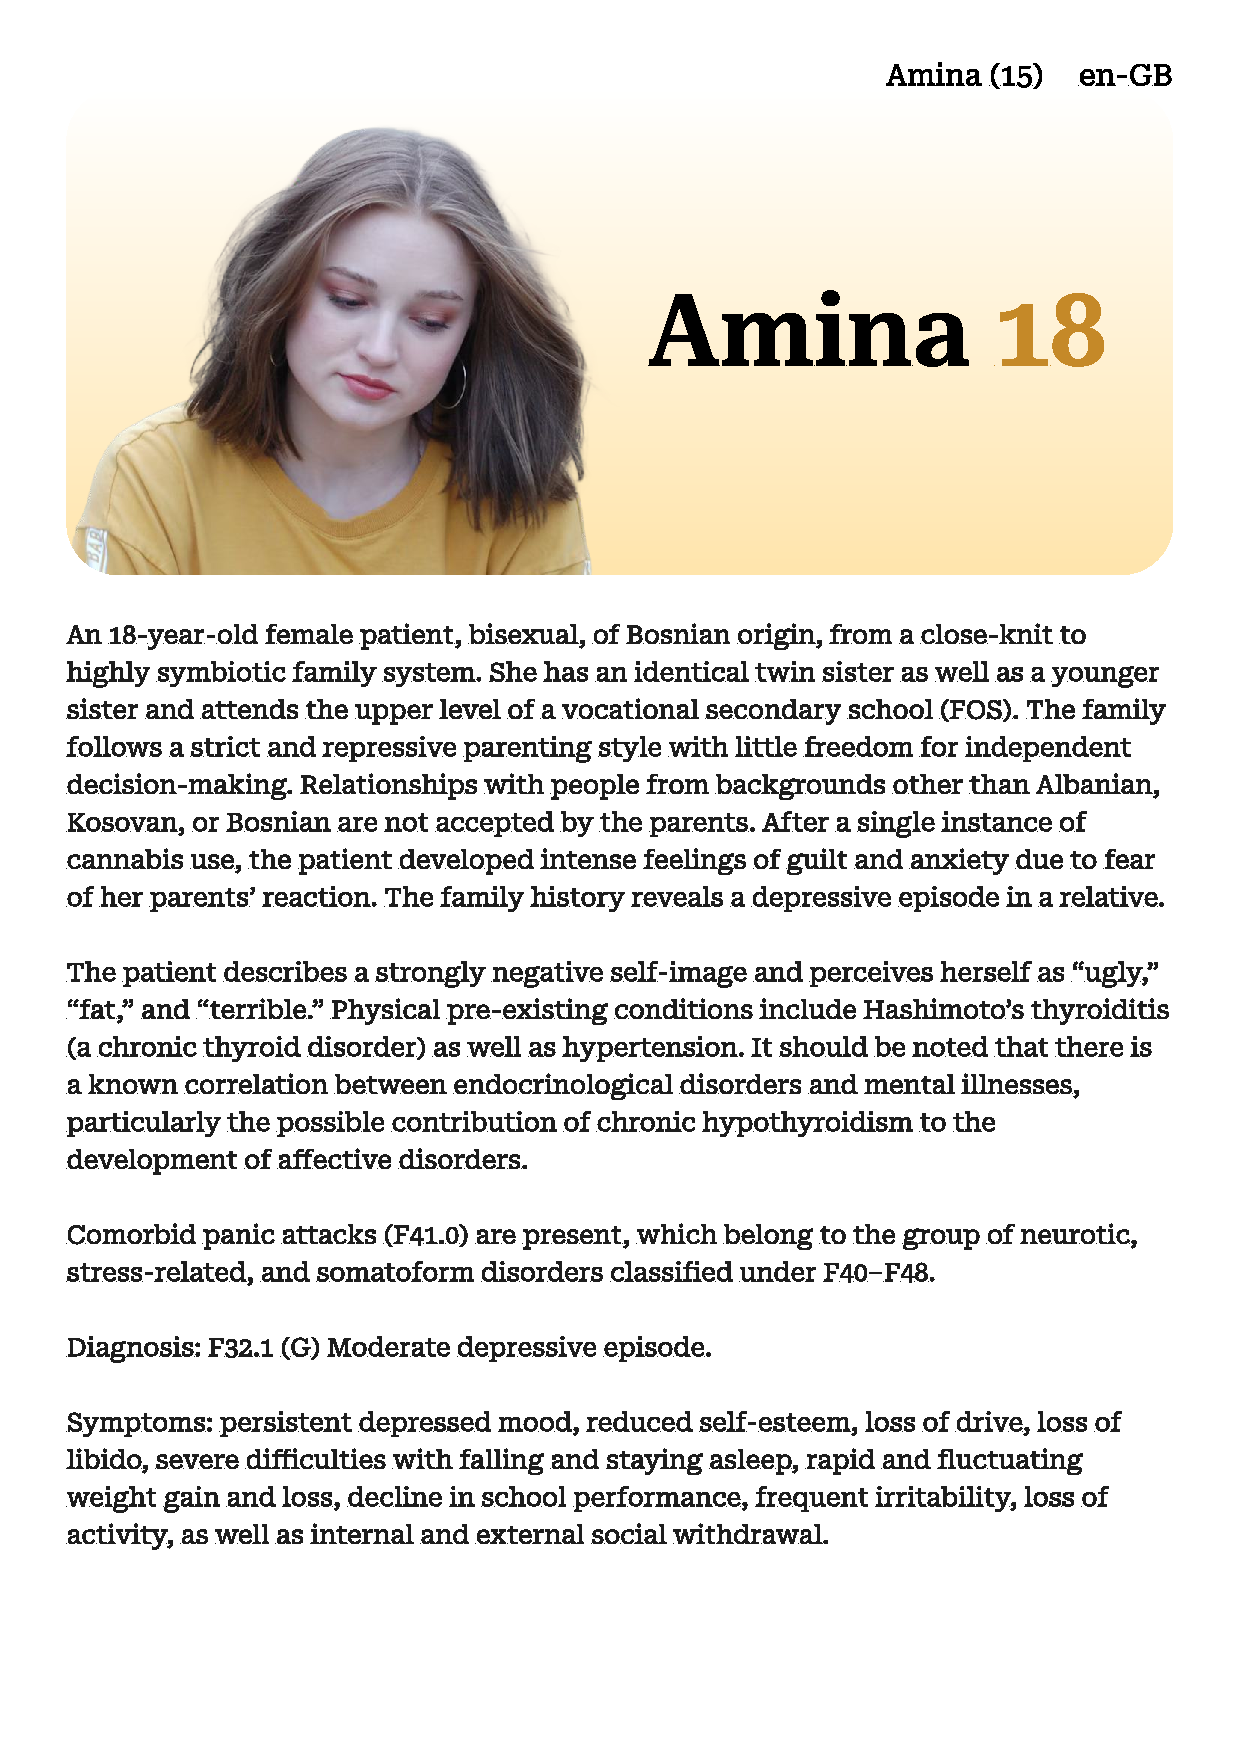
\includegraphics[page=1,width=.3\textwidth]{assets/vignettes/Amina-en-GB.pdf}
 \caption{Amina}
 \label{fig:app:Amina}
\end{figure}
\begin{figure}[H]
   \centering
   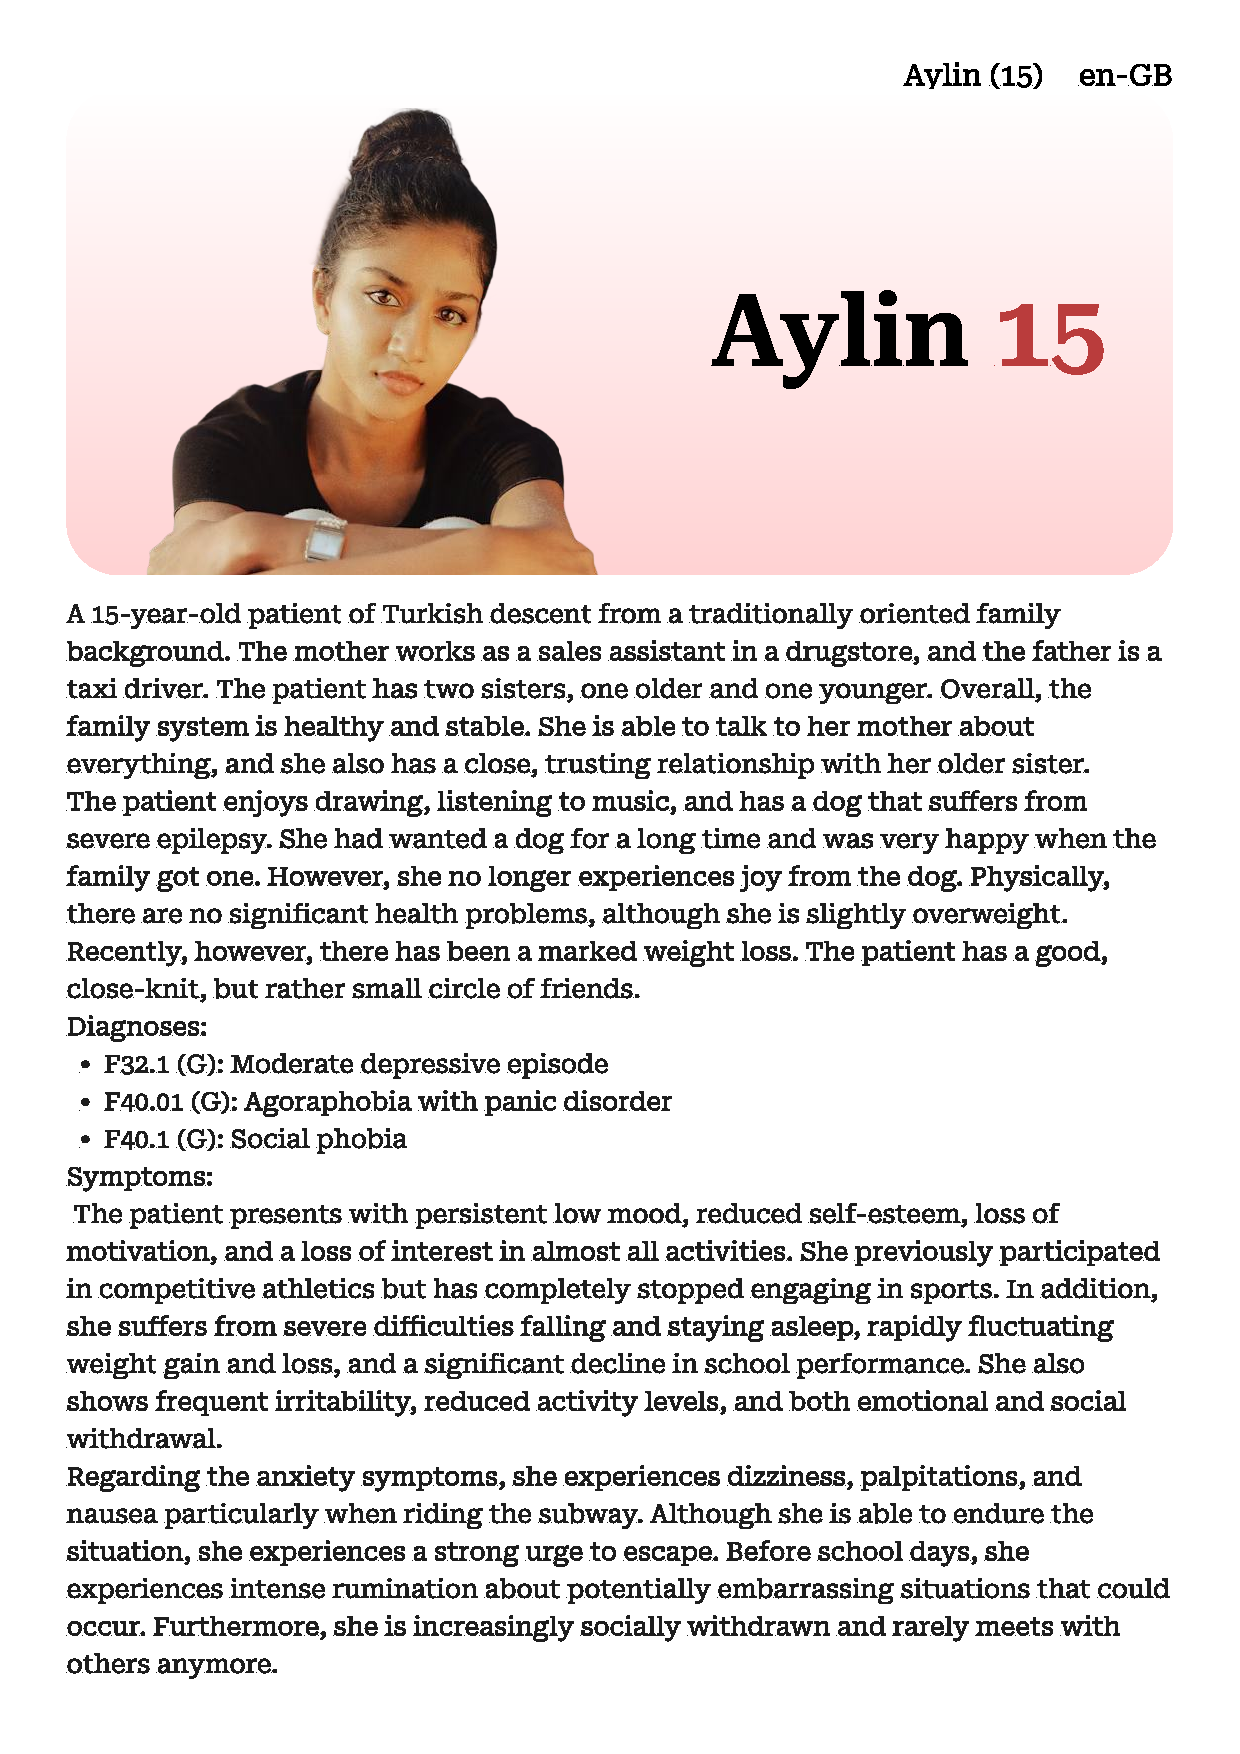
\includegraphics[page=1,width=.3\textwidth]{assets/vignettes/Aylin-en-GB.pdf}
 \caption{Aylin}
 \label{fig:app:Aylin}
\end{figure}
\begin{figure}[H]
   \centering
   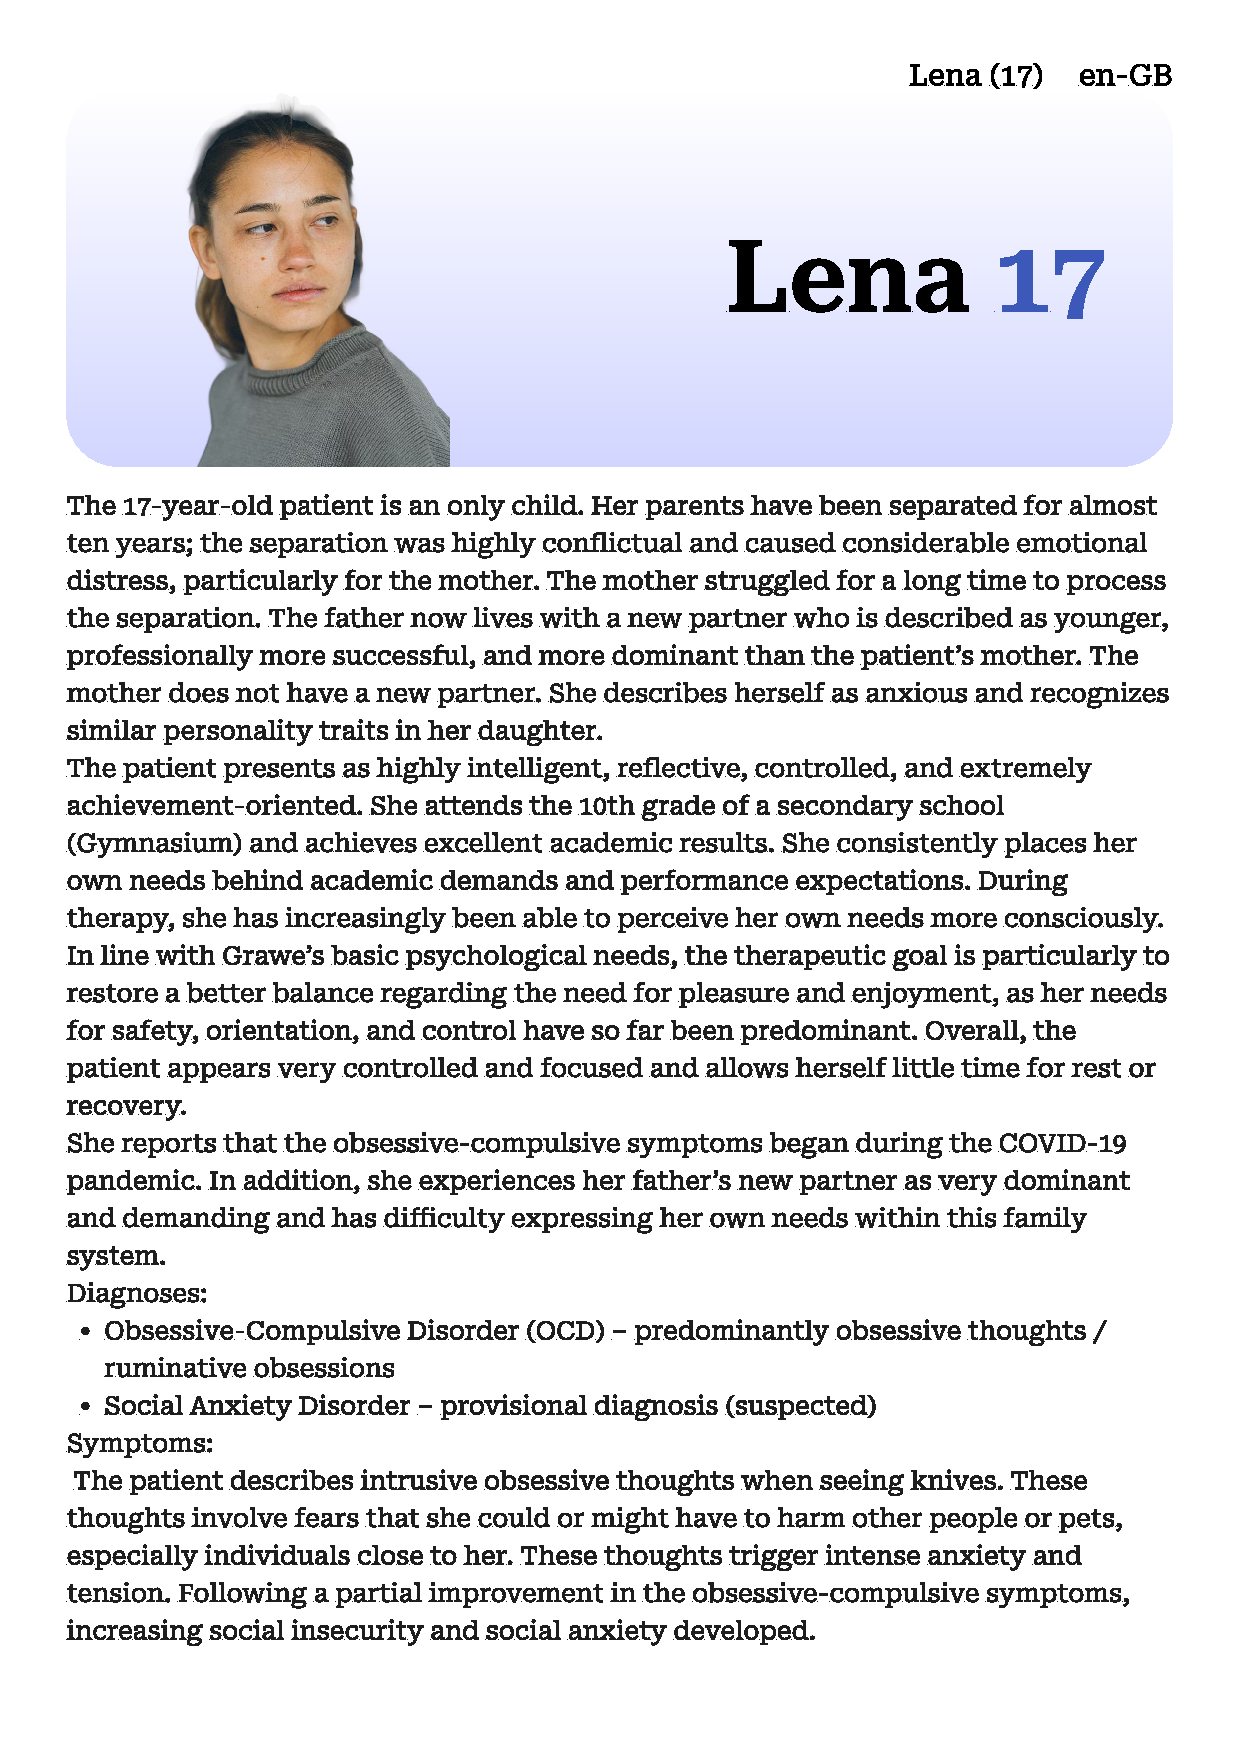
\includegraphics[page=1,width=.3\textwidth]{assets/vignettes/Lena-en-GB.pdf}
 \caption{Lena}
 \label{fig:app:Lena}
\end{figure}
\begin{figure}[H]
   \centering
   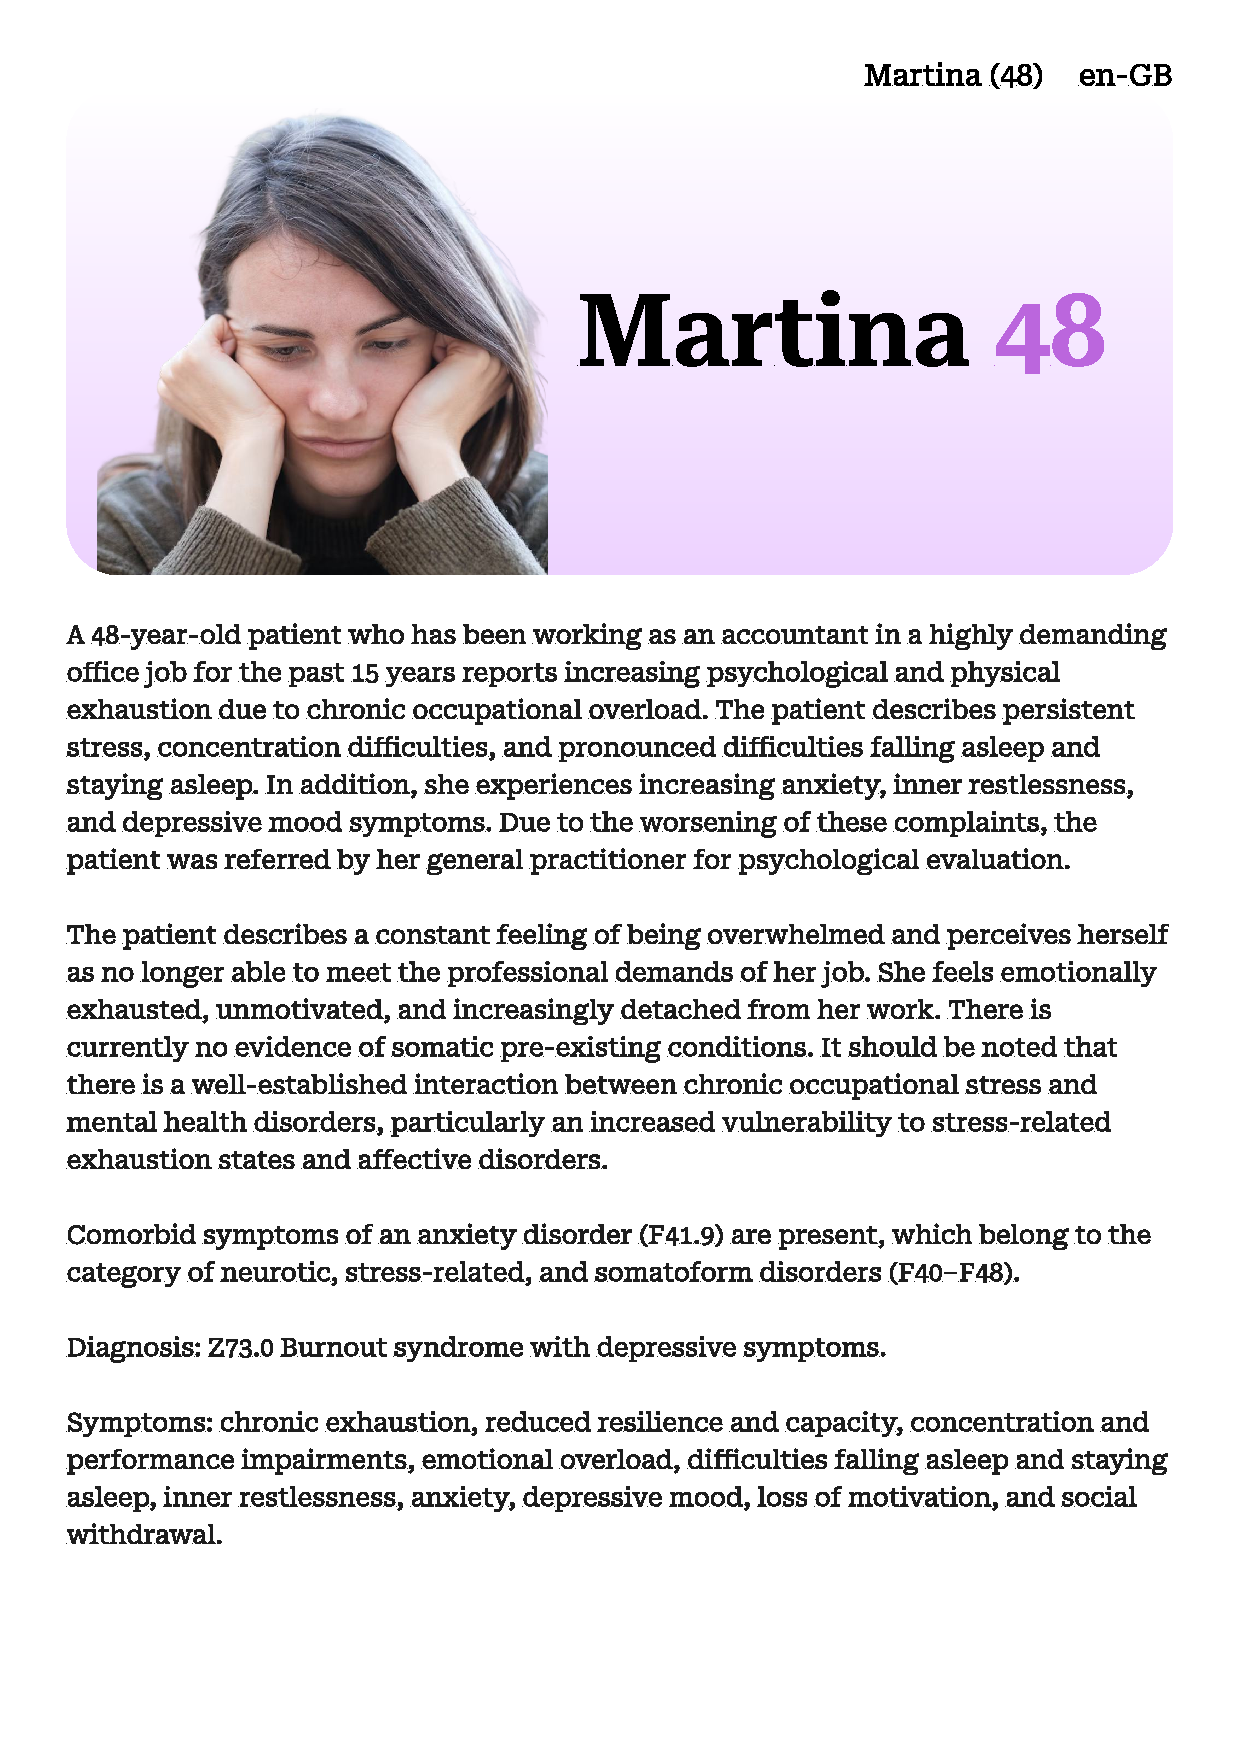
\includegraphics[page=1,width=.3\textwidth]{assets/vignettes/Martina-en-GB.pdf}
 \caption{Martina}
 \label{fig:app:Martina}
\end{figure}
\begin{figure}[H]
   \centering
   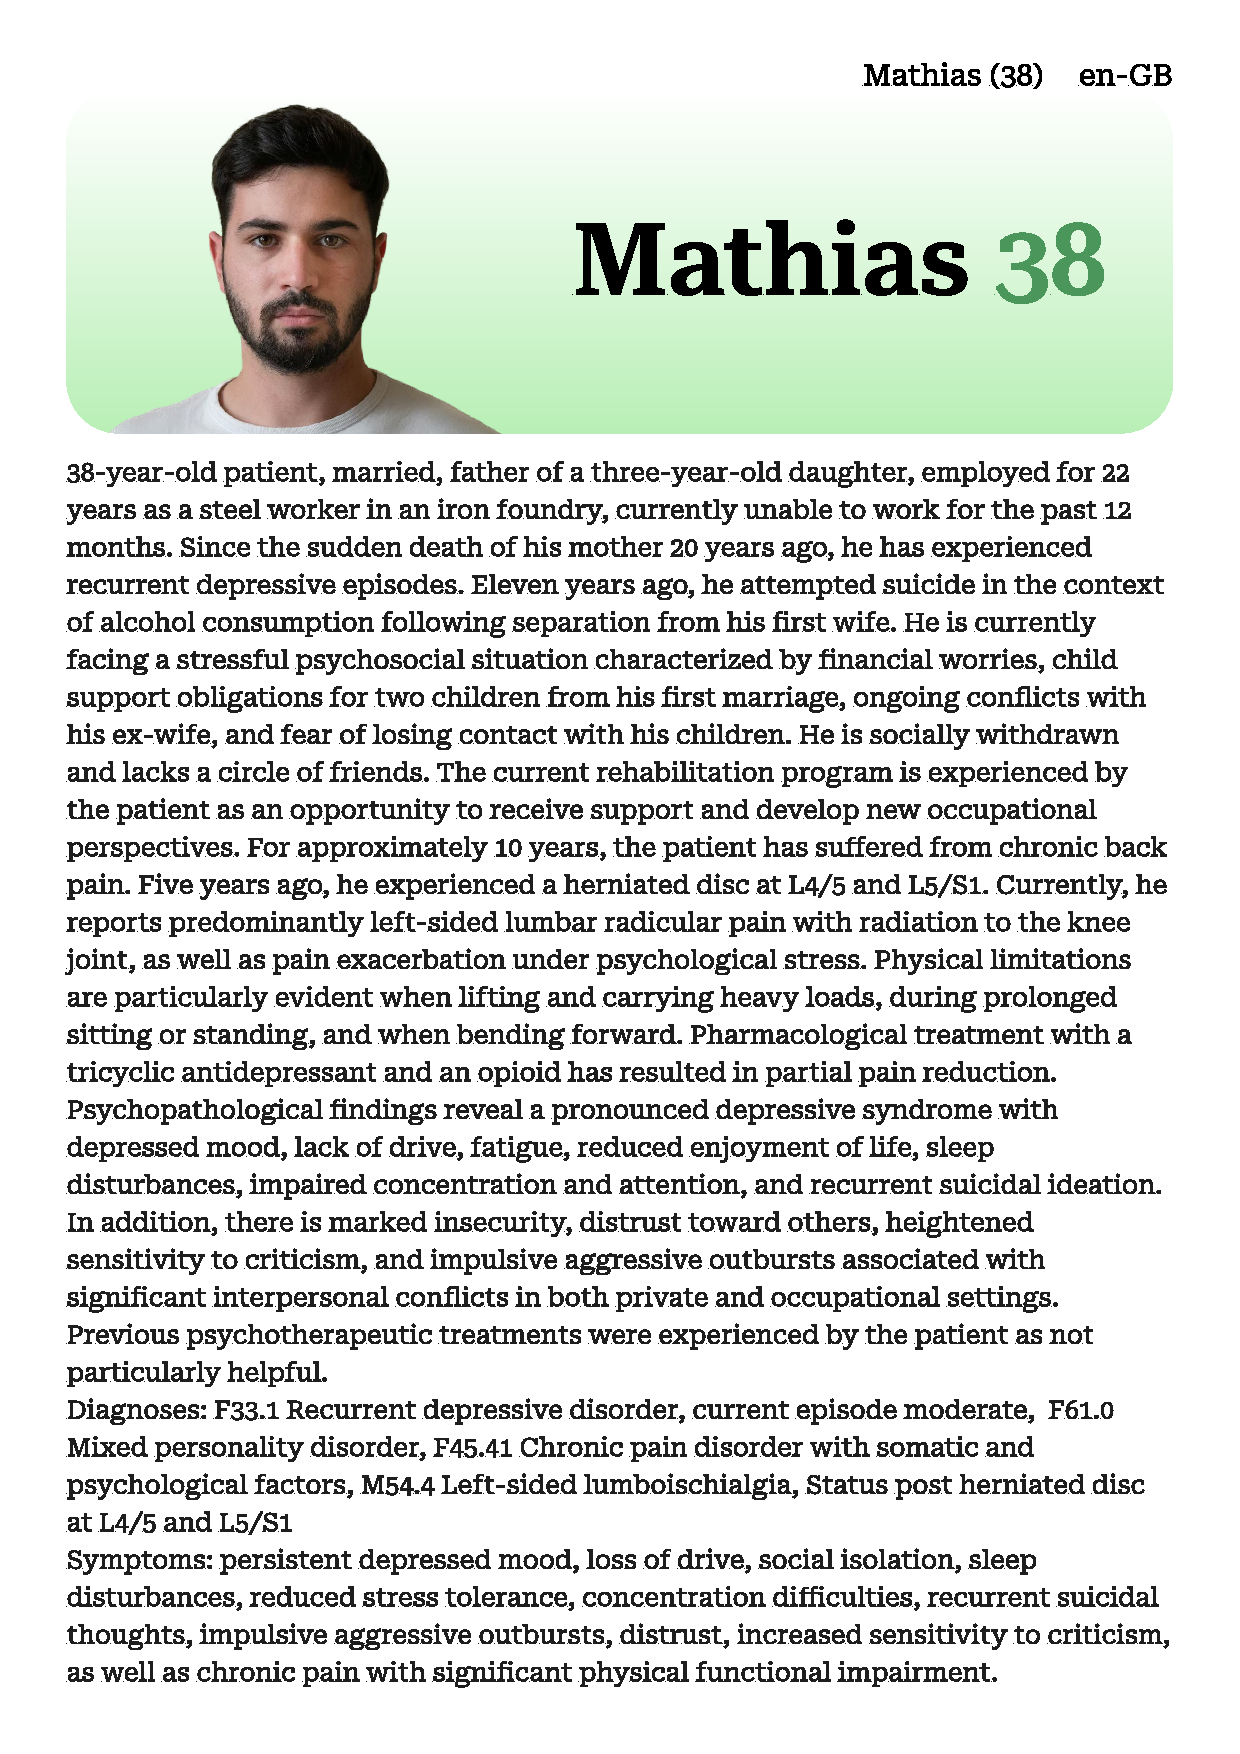
\includegraphics[page=1,width=.3\textwidth]{assets/vignettes/Mathias-en-GB.pdf}
 \caption{Mathias}
 \label{fig:app:Mathias}
\end{figure}

\subsection{Plots}
\begin{figure}[H]

    \centering

    \begin{subfigure}{0.48\linewidth}
        \centering
        
\includegraphics[width=\linewidth]{assets/graphs/active.png}
        \caption{Active}
        \label{fig:app:active}
    \end{subfigure}
    \hfill
    \begin{subfigure}{0.48\linewidth}
        \centering
        
\includegraphics[width=\linewidth]{assets/graphs/control.png}
        \caption{Control}
        \label{fig:app:control}
    \end{subfigure}

    \caption{Comparison of Active and Control conditions.}
    \label{fig:app:active-control}
\end{figure}

\begin{figure}[H]
    \centering

    \begin{subfigure}{0.48\linewidth}
        \centering
        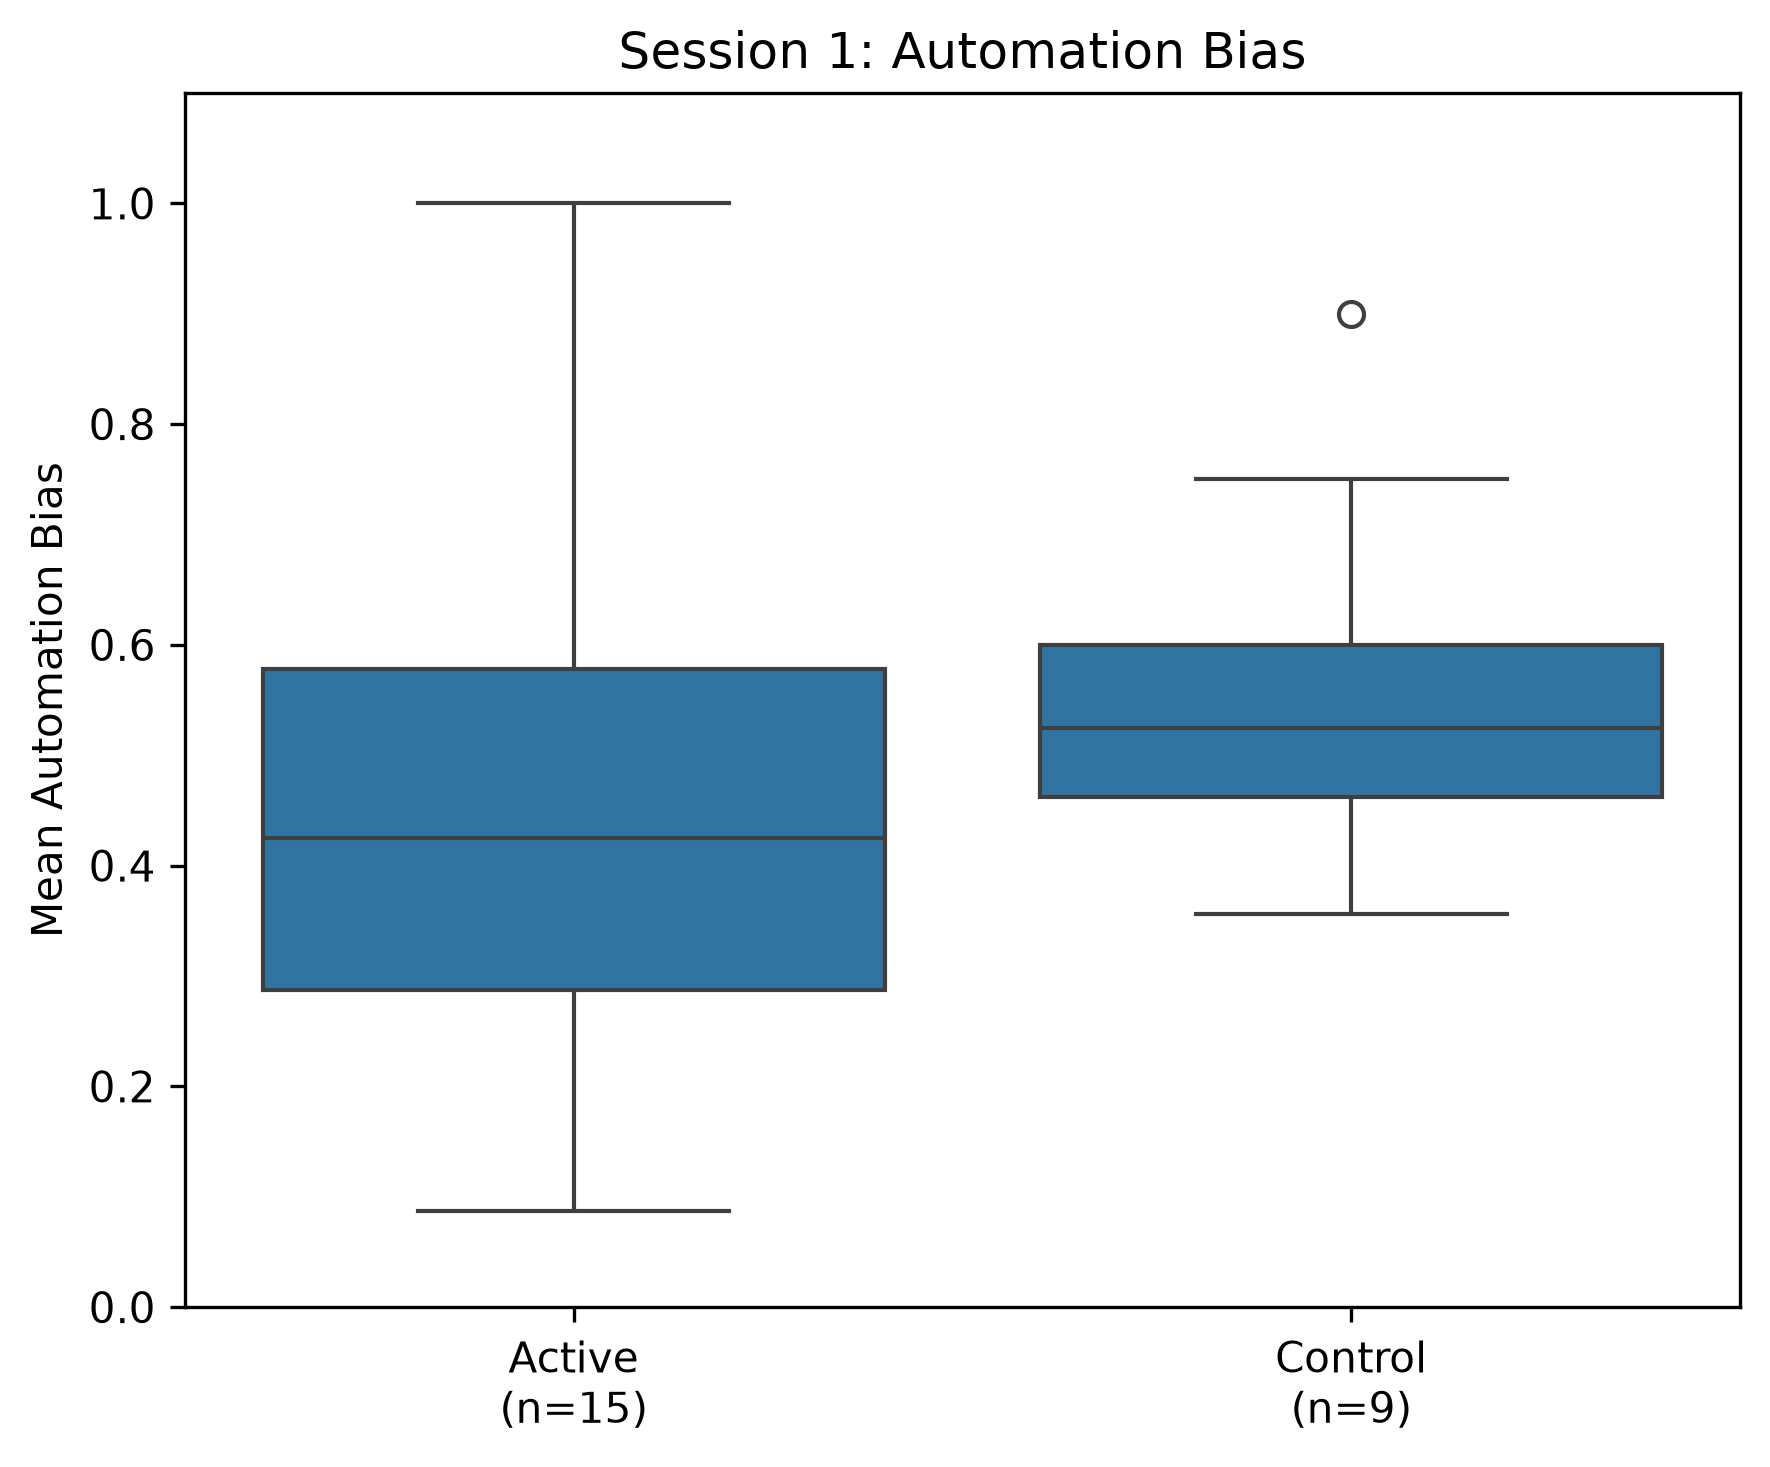
\includegraphics[width=\linewidth]{assets/graphs/session1.png}
        \caption{Session 1}
        \label{fig:app:session1}
    \end{subfigure}
    \hfill
    \begin{subfigure}{0.48\linewidth}
        \centering
        
\includegraphics[width=\linewidth]{assets/graphs/session2.png}
        \caption{Session 2}
        \label{fig:app:session2}
    \end{subfigure}

    \caption{Comparison of Session 1 and Session 2.}
    \label{fig:app:sessions}
\end{figure}


\subsection{PWA}
\label{app:pwa}
\begin{figure}[H]
    \centering

    \begin{subfigure}{\textwidth/7}
        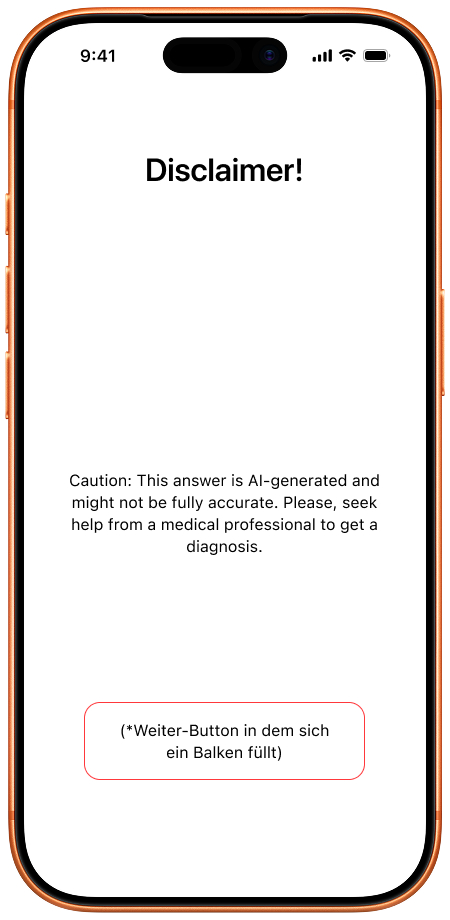
\includegraphics[width=\linewidth]{assets/Design/Disclaimer.jpg}
        \caption{Disclaimer}
    \end{subfigure}
    \begin{subfigure}{\textwidth/7}
        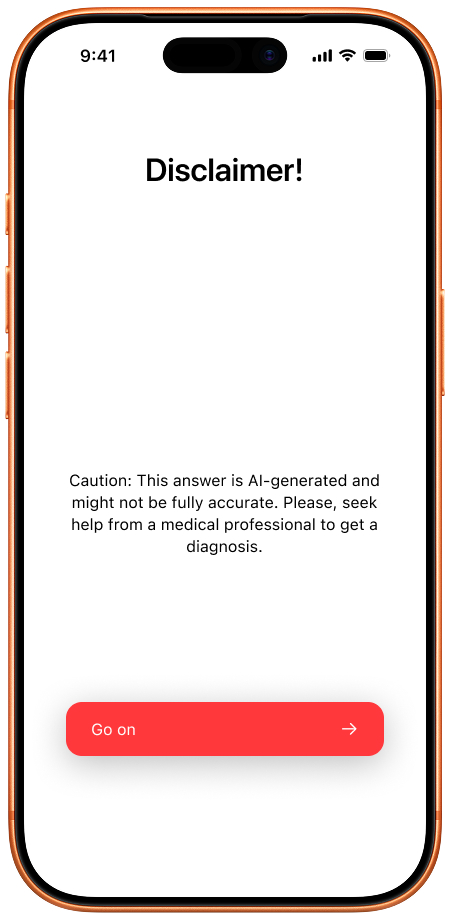
\includegraphics[width=\linewidth]{assets/Design/Disclaimer 2.jpg}
        \caption{Disclaimer done}
    \end{subfigure}
    \begin{subfigure}{\textwidth/7}
        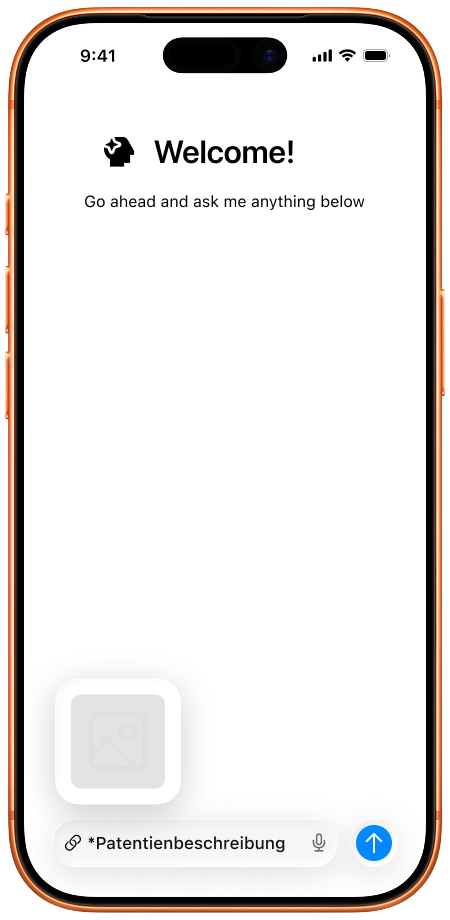
\includegraphics[width=\linewidth]{assets/Design/Auto Eingabe.jpg}
        \caption{Prompt}
    \end{subfigure}
    \begin{subfigure}{\textwidth/7}
        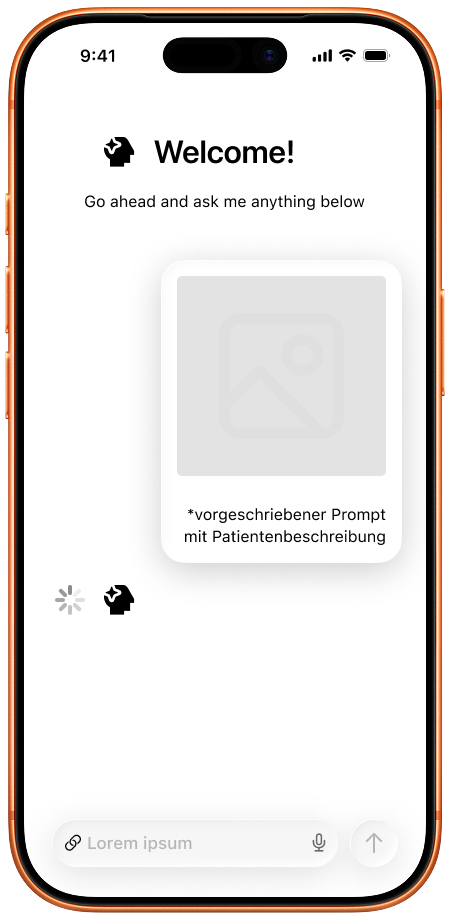
\includegraphics[width=\linewidth]{assets/Design/Senden.jpg}
        \caption{Sent}
    \end{subfigure}
    \begin{subfigure}{\textwidth/7}
        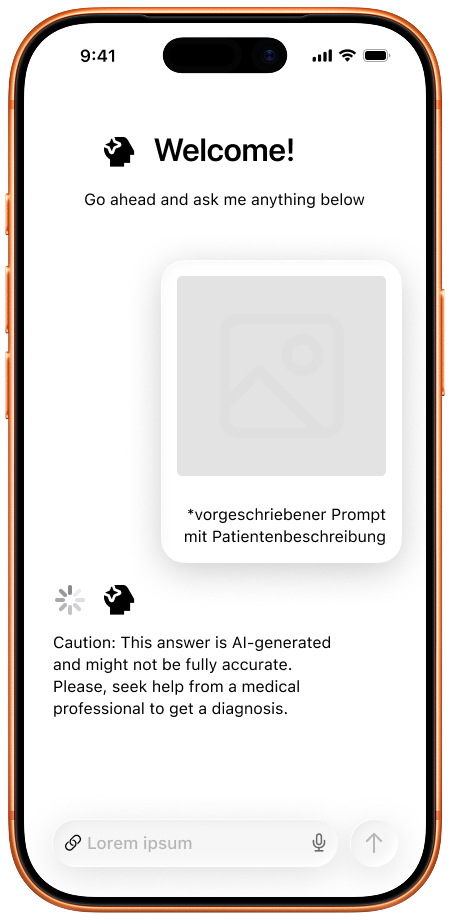
\includegraphics[width=\linewidth]{assets/Design/Disclaimer Inline.jpg}
        \caption{Inline Disclaimer}
    \end{subfigure}
    \begin{subfigure}{\textwidth/7}
        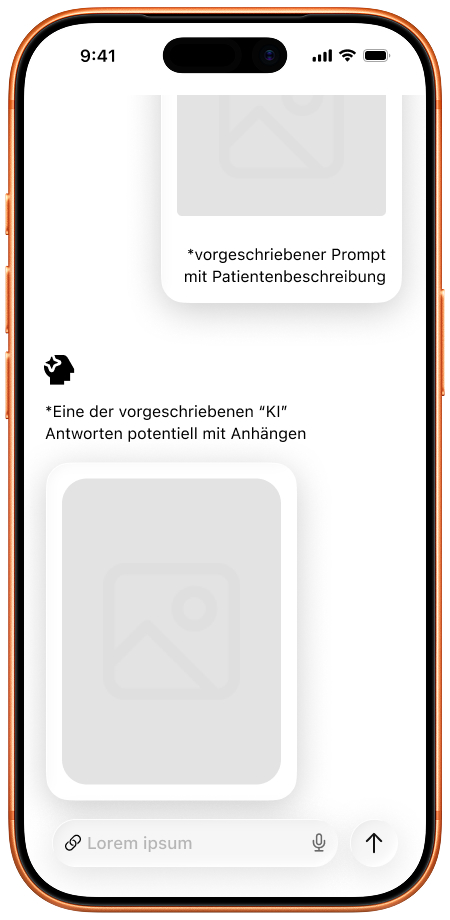
\includegraphics[width=\linewidth]{assets/Design/Result.jpg}
        \caption{Response}
    \end{subfigure}

    \caption{App Design in Figma}
    \Description{Six screens we designed in the ideation phase for our testing application.}
    \label{fig:app:design}
\end{figure}
